\documentclass[11pt]{article}
\usepackage{minted}
\usepackage{classTools}
\usepackage{xcolor}
\usepackage{graphicx}
\graphicspath{ {./graphs/} }

\begin{document}

\psHeader{1}{Wed 2023-09-20 (11:59pm)}

Please review the Syllabus for information on the collaboration policy, grading scale, revisions, and late days.


\begin{enumerate}
    \item (Asymptotic Notation) 
    \begin{enumerate}
    \item (practice using asymptotic notation)
        Fill in the table below with ``T'' (for True) or ``F'' (for False) to indicate the relationship between $f$ and $g$. For example, if $f$ is $O(g)$, the first cell of the row should be ``T.'' \\
        \begin{table}[h!]
        \centering
        \bgroup
        \def\arraystretch{1.3}
        \begin{tabular}{||c | c || c | c | c | c | c ||}
         \hline
         $f$ & $g$ & $O$ & $o$ & $\Omega$ & $\omega$ & $\Theta$ \\
         \hline\hline
         $e^{n^2}$ & $e^{2n^2}$ & T & T & F & F & F \\ \hline
         $n^3$ & $n^{3/n}$ & F & F & T & T & F \\ \hline
         $n^{2+(-1)^n}$ & $\binom{n}{2}$ & F & F & F & F & F \\ \hline
         $(\log {n})^{120}\sqrt{n}$ & $n$ & F & F & T & T & F \\ \hline
         $\log(e^{n^2})$ & $\log(e^{2n^2})$ & T & F & T & F & T \\ \hline
        \end{tabular}
        \egroup
        \end{table}
        Recall that, throughout CS120, all logarithms are base 2 unless otherwise specified. 
        
    \item  (rigorously reasoning about asymptotic notation)  
    For each of the following claims, either justify why the statement holds (for all $f$, $g$) or provide a counterexample. In all cases, take the domain of the functions $f$ and $g$ to be the natural numbers (rather than the positive reals), and assume $f(n), g(n)\geq 1$ for all $n$.
    \begin{itemize}
        \item For all positive integers $a$ and $b$, if $f(n) = \Theta(a^n)$ and $g(n) = \Theta(n^b)$, then $f(g(n)) = \Theta(a^{(n^b)})$.
        \begin{quote}
            \color{purple}
            The claim is false. Consider this counter example.

            Begin by introducing valid variables assignments for the counter example:
            \begin{itemize}
                \item Let $a = b = 2$
                \item Let $c_0 = c_1 = c_2 = c_3 = 4$
            \end{itemize}
            In this example, let $f(n) = 4 \cdot 2^n$ and let $g(n) = 4 \cdot n^2$. \newline
            The definition of $f(n)$ is a valid case of $f(n) = \Theta(a^n)$ because there are nonzero constants $c_0$ and $c_1$ such that 
            $$c_0 \cdot a^n = 4 \cdot 2^n \leq f(n) = 4 \cdot 2^n \leq 4 \cdot 2^n = c_1 \cdot a^n$$ 
            for all great-enough $n$. \newline
            Similarly, the definition of $g(n)$ is a valid case of $g(n) = \Theta(n^b)$ because there are nonzero constants $c_2$ and $c_3$ such that 
            $$c_2 \cdot n^b = 4 \cdot n^2 \leq g(n) = 4 \cdot n^2 \leq 4 \cdot n^2 = c_3 \cdot n^b$$ \newline
            Combining these valid definitions of $f(n)$ and $g(n)$, let $f(g(n)) = 4 \cdot 2^{4 \cdot n^2}$. \newline
            For $f(g(n) = \Theta(a^{(n^b)})$ to be true, $4 \cdot 2^{4 \cdot n^2}$ must be both $O(a^{(n^b)})$ and $\Omega(a^{(n^b)})$. Begin by testing $O(a^{(n^b)} = 2^{n^2})$. \newline
            For $4 \cdot 2^{4 \cdot n^2} = O(2^{n^2})$ to be true, there must exist some constant $c_k$ such that $4 \cdot 2^{4 \cdot n^2} \leq c_k \cdot 2^{n^2}$ for all large-enough $n$. \newline
            Algebraically manipulate this inequality: 
            \begin{align*}
                && 4 \cdot 2^{4 \cdot n^2} \leq c_k \cdot 2^{n^2} && \text{Initial} && \\
                && 4 \cdot 16^{n^2} \leq c_k \cdot 2^{n^2} && \text{Apply exponent} &&  \\
                && 4 \cdot 2^{n^2} \cdot 8^{n^2} \leq c_k \cdot 2^{n^2} && \text{Break apart $16^{n^2}$} &&  \\
                && 4 \cdot 8^{n^2} \leq c_k && \text{Divide both sides by $2^{n^2}$} &&  \\
            \end{align*}
            Considering the final inequality, there is no constant $c_k$ such that the inequality is true for all arbitrarily-large $n$. Because the inequality must be false, $4 \cdot 2^{4 \cdot n^2} \neq O(2^{n^2})$. Because the valid construction of $f(g(n))$ is not $O$ of $n$, it also cannot be $\Theta$ of $n$. By this counter example, the claim is disproved.
        \end{quote}
        \item For all positive integers $a$ and $b$, if $f(n) = \Theta(a^n)$ and $g(n) = \Theta(n^b)$, then $g(f(n)) = \Theta((a^n)^b)$.
        \begin{quote}
            \color{purple}
            I will prove the claim directly by constructing a valid and exhaustive definition of $g(f(n))$ and then examining two cases about its relationship with $(a^n)^b$. \newline 
            Assume there exist functions $f(n)$ and $g(n)$ such that $f(n) = \Theta(a^n)$ and $g(n) = \Theta(n^b)$ for all positive integers $a$ and $b$. \newline
            By these definitions, there exist nonzero constants $c_0$, $c_2$, $c_3$, and $c_5$ such that 
            $$c_0 \cdot a^n \leq f(n) \leq c_2 \cdot a^n$$
            and
            $$c_3 \cdot n^b \leq g(n) \leq c_5 \cdot n^b$$
            Let $f(n)$ be defined as $f(n) = c_1 \cdot a^n$ where $c_1$ is any nonzero constant that satisfies the inequality for $f(n)$. \newline 
            Similarly, let $g(n)$ be defined as $g(n) = c_4 \cdot n^b$ where $c_4$ is any nonzero constant that satisfies the inequality for $g(n)$. \newline
            By these definitions, let $g(f(n)) = c_4 \cdot (c_1 \cdot a^n)^b$. For $c_4 \cdot (c_1 \cdot a^n)^b = \Theta((a^n)^b)$ to be true, $c_4 \cdot (c_1 \cdot a^n)^b$ must be both $O$ and $\Theta$ of $(a^n)^b$. Prove these cases separately: \newline
            \newline 
            \textbf{Prove $c_4 \cdot (c_1 \cdot a^n)^b = O((a^n)^b)$}: \newline
            For this sub-claim to be true, there must exist some nonzero constant $c_k$ such that $c_4 \cdot (c_1 \cdot a^n)^b \leq c_k \cdot (a^n)^b$. Simplify this equality to examine its correctness:
            \begin{align*}
                && c_4 \cdot (c_1 \cdot a^n)^b \leq c_k \cdot (a^n)^b && \text{Initial} && \\
                && c_4 \cdot (c_1)^b \cdot a^{n \cdot b} \leq c_k \cdot a^{n \cdot b} && \text{Apply exponent} && \\
                && c_4 \cdot (c_1)^b \leq c_k && \text{Divide both sides by $a^{n \cdot b}$} && \\
            \end{align*}
            Because $c_4$, $c_1$, and $b$ are constants, it's guaranteed that some $c_k$ exists such that $c_4 \cdot (c_1)^b \leq c_k$ is true. This confirms that $c_4 \cdot (c_1 \cdot a^n)^b = O((a^n)^b)$. \newline
            \newline
            \textbf{Prove $c_4 \cdot (c_1 \cdot a^n)^b = \Omega((a^n)^b)$}: \newline
            For this sub-claim to be true, there must exist some nonzero constant $c_k$ such that $c_4 \cdot (c_1 \cdot a^n)^b \geq c_k \cdot (a^n)^b$. Without repeating the algebraic simplifications from the proof for $O$, assert that the final inequality can be properly reused in this proof with a reversed operator such that $c_4 \cdot (c_1)^b \geq c_k$. \newline 
            Again, because $c_4$, $c_1$, and $b$ are all nonzero constants, it's guaranteed that some $c_k$ exists such that $c_4 \cdot (c_1)^b \geq c_k$ is true. This confirms that $c_4 \cdot (c_1 \cdot a^n)^b = \Omega((a^n)^b)$.
            \newline 
            \newline 
            Because a valid, exhaustive definition of $g(f(n))$ is both $O$ and $\Omega$ of $(a^n)^b$, the claim must be true and $g(f(n)) = \Theta((a^n)^b)$.
        \end{quote}
    \end{itemize}
  
    \end{enumerate}
    
    \newpage
    
    \item (Understanding computational problems and mathematical notation)\\\\
    Recall the definition of a {\em computational problem} from Lecture Notes 1.  

 
    Consider the following computational problem $\Pi=(\Inputs,\Outputs,f)$ and algorithm $\BC$ to solve it, where
    \begin{itemize}                                
    \item $\Inputs = \N\times\N\times \N$ 
    \item $\Outputs = \{(c_0,c_1,\ldots,c_{k-1}) : k,c_0,\ldots,c_{k-1}\in \N\}$
    \item $f(n,b,k) = \{ (c_0,c_1,\ldots,c_{k-1}) : n=c_0+c_1b+c_2b^2+\cdots+c_{k-1}b^{k-1}, \forall i\ 0\leq c_i< b\}.$ 
    \end{itemize}

    
\begin{algorithm}[H]
    \BC{$n,b,k$}\\
    {
    \lIf{$b<2$}{\Return{$\bot$}}
    \ForEach{$i=0,\ldots,k-1$}{
    $c_i = n \bmod b$\;
    $n = (n-c_i)/b$\;
    }
    \lIf{$n==0$}{\Return{$(c_0,c_1,\ldots,c_{k-1})$}}
    \lElse{\Return{$\bot$}}}
\end{algorithm}


\begin{enumerate}
\item If the input is $(n,b,k) = (11,10,4)$, what does the algorithm BC return? (Note that the output is not (1,1).) Is BC's output a valid solution for $\Pi$ with input $(11,10,4)$?
    \begin{quote}
        \color{purple}
        Given input $(n, b, k) = (11, 10, 4)$, \BC outputs $c = (c_0, c_1, c_2, c_3) = (1, 1, 0, 0)$.
        Here's why it's valid:
        \begin{itemize}
            \item $c$ has $k$ elements.
            \item Given $b = 10$ as input, $c_0 + c_1b + ... = 1 + 1 \cdot 10 + 0 \cdot 10^2 + 0 \cdot 10^3 = 11 = n$.
            \item Every $c_i$ in $c$ is in the range $0 \leq c_i < b = 10$.
        \end{itemize}
    \end{quote}
\item Describe the computational problem $\Pi$ in words.  (You may find it useful to try some more examples with $b=10$.) 
    \begin{quote}
        \color{purple}
        $\BC$ is a function for converting base-10 numbers to different base systems. For example, the triple $(n, b, k) = (11, 10, 4)$ is asking to convert the number $11$ to base $10$ with space for at-most $4$ output digits. If we reverse the output $(1, 1, 0, 0)$, the result is $0011$, which indeed is the base-10 number $11$ with four digits of precision. For a further example, consider input $(19, 2, 8)$. The output, reversed and condensed as $00010011$, is the number $19$ in binary with eight digits of precision. The converter takes in any triple of natural numbers and returns either nothing or the calculated sequence of values. Of note, if $k$ is not long enough, output will not be a valid conversion (this case is caught by the final return statement).
    \end{quote}
\item Is there any $x\in \Inputs$ for which $f(x)=\emptyset$? If so, give an example; if not, explain why.
    \begin{quote}
        \color{purple}
        Yes. A non-empty return type from $\BC$ should contain a tuple of length $k$. However, if a conversion into base-1 is requested, $b = 1$, function $\BC$ has no viable result and simply returns $\bot$. A similar case occurs when a base conversion is requested but the $k$ provided is too small to hold the output.
    \end{quote}
\item For each possible input $x\in \Inputs$, what is $|f(x)|$? ($|A|$ is the size of a set $A$.) Justify your answer(s) in one or two sentences.
    \begin{quote}
        \color{purple}
        The size of $f(x)$ is either one or zero. If the algorithm returns $\bot$, $f(x) = \emptyset$. If the algorithm does not return $\bot$, it returns a single tuple representing the converted number. Conversion is deterministic, so there is no variation in the contents of this returned tuple.
    \end{quote}
\item Let $\Pi'=(\Inputs,\Outputs,f')$ be the problem with the same $\Inputs$ and $\Outputs$ as $\Pi$, but $f'(n,b,k) = f(n,b,k) \cup \{(0,1, \ldots,k-1)\}$. Does every algorithm $A$ that solves $\Pi$ also solve $\Pi'$? (Hint: any differences between inputs that were relevant in the previous subproblem are worth considering here.) Justify your answer with a proof or a counterexample.
    \begin{quote}
        \color{purple}
        The claim is false. Let there be some $x$ such that $f(x) = \emptyset$ (ex. requested conversion into base 1 or not enough space for a valid output). In this case, $f'(x) = {(0, 1, ..., k - 1)}$ because of the set union. So, the expected output of $f'(x)$ is different from the expected output of $f(x)$. Because of this, not every algorithm A that solves $\Pi$ also solves $\Pi'$.
    \end{quote}

\end{enumerate}
\newpage

\item (Radix Sort) In the Sender--Receiver Exercise associated with lecture 3, you studied the sorting algorithm {\em Counting Sort}, generalized to arrays of key--value pairs, and proved that it has running time $O(n+U)$ when the keys are drawn from a universe of size $U$. In this problem you'll study {\em Radix Sort}, which improves the dependence on the universe size $U$ from linear to logarithmic.  Specifically, Radix Sort can achieve runtime $O(n+n(\log U)/(\log n))$, so it achieves runtime $O(n)$ whenever $U = n^{O(1)}$.  
Radix Sort is constructed by using Counting Sort as a subroutine several times, but on a smaller universe size $b$.
Crucially, Radix Sort uses the fact that Counting Sort can be implemented in a way that is {\em stable} in the sense that it preserves the order in the input array when the same key appears multiple times.  Here is pseudocode for Radix Sort, using the algorithm $BC$ above as a subroutine:

\begin{algorithm}[H]
\RadixSort{$U,b,A$}\\
\Input{A universe size $U\in \N$, a base $b\in \N$ with $b\geq 2$, and an array $A=((K_0,V_0),\ldots,(K_{n-1},V_{n-1}))$, where each $K_i\in [U]$}
\Output{A valid sorting of $A$}
$k=\lceil (\log U)/(\log b)\rceil$\;
\ForEach{$i=0,\ldots,n-1$}{
    $V_i' = \BC(K_i,b,k)$}
\ForEach{$j=0,\ldots,k-1$}{
    \ForEach{$i=0,\ldots,n-1$}{
    $K'_i = V'_i[j]$
    }
    $((K_0',(V_0,V'_0)),\ldots,(K_{n-1}',(V_{n-1},V'_{n-1}))) = \CountingSort(b,((K'_0,(V_0,V_0')),\ldots,(K'_{n-1},(V_{n-1},V'_{n-1})))$\;
}
\ForEach{$i=0,\ldots,n-1$}{
    $K_i = V'_i[0]+V'_i[1]\cdot b + V'_i[2]\cdot b^2+\cdots+V'_i[k-1]\cdot b^{k-1}$}
\Return{$((K_0,V_0),\ldots,(K_{n-1},V_{n-1}))$}
\caption{Radix Sort}
\end{algorithm}

(You can also read a description of Radix Sort in CLRS Section 8.3 for the case of sorting arrays of keys (without attached items) when $U$ and $b$ are powers of 2, albeit using different notation than us.)

        \begin{enumerate}
        
            \item (proving correctness of algorithms) Prove the correctness of \RadixSort\ (i.e. that it correctly solves the Sorting problem). 
            
            Hint: You will need to use the stability of \CountingSort in your argument. Note that if in the 8th line of \RadixSort algorithm, you replaced \CountingSort with ExhaustiveSearchSort (or any other sort which isn't stable), the resulting algorithm would not correctly solve sorting. 

            Here is an example (using ExhaustiveSearchSort instead of stable sort in line 8). Suppose $n=3, b=2, U=4$, $K_0=1, K_1=3, K_2=2$ and $V_0, V_1, V_2$ are ``a'', ``b'', and ``c''. Then $V'_0=(1,0), V'_1=(1,1), V'_2=(0,1)$. Suppose ExhaustiveSearchSort is such that the permutation $\pi(2)=0, \pi(1)=1, \pi(0)=2$ 
 is tried first. Sorting based on the first bit will lead to the array $(K_2=2, (c,(0,1))), (K_1=3, (b,(1,1))), (K_0=1,(a,(1,0)))$. Next, sorting the second bit using the same ExhaustiveSearchSort will give the array $(K_0=1,(a,(1,0))), (K_1=3, (b,(1,1))), (K_2=2, (c,(0,1)))$. Thus we return the same input array $((1,a),(3,c),(2,b))$!
    \begin{quote}
        \color{purple}
        I will prove the correctness of $\RadixSort$ by applying induction on variable $j$ in the given pseudocode. Begin by clarifying key elements of the algorithm: \newline
        The value $k$ is the greatest number of digits in base $b$ of any input key. For example, given input $A$ with keys $[9, 90, 900]$, the value of $k$ in base 10 will be $3$. \newline 
        In $\RadixSort$, the input elements are transformed into sort keys by splitting and reversing their base $b$ representations. For example, the input key $900$ in base 10 is indexed as length-$k$ collection of sort keys $[0, 0, 9]$. \newline 
        The iteration integer $j$ ascends from $0$ to $k - 1$ such that the there are $k$ total sort keys for every input key. Again using $900$ as an example, valid sort keys at $j = 0$, $j = 1$, and $j = 2$ are $0$, $0$, and $9$ respectively. \newline
        Applying these definitions, consider the following inductive argument on any $n \geq 0$ key-value pairs of input as defined by the sorting problem: 
        \newline
        \newline 
        \textbf{Edge case}: $k = 0$ \newline
        There is no input to be sorted. So, the (empty) output of $\RadixSort$ will be a sorted permutation of the (empty) input.
        \newline 
        \newline
        \textbf{Base case}: $k = 1$ \newline
        When $k = 1$, iteration for $j$ only passes through the input once. Because the entirety of every sort key is evaluated by $\CountingSort$, the output of $\RadixSort$ is the output of $\CountingSort$, which is a valid solution to the sorting problem.
        \newline 
        \newline
        \textbf{Inductive hypothesis}: \newline 
        Given input of length $n$ with some $k \geq 1$, assume the input has been properly sorted by the first $k - 2 = j$ sort key indices. \newline
        \newline
        \textbf{Inductive step}: \newline 
        Prove the correctness after sorting on the $j + 1$ sort key. \newline 
        At this step, counting sort will sort each element by only its $j + 1$ sort key. Consider the sorting of any two sort keys $\alpha$ and $\beta$ representing the $j + 1$ sort key of two different input keys: 
        \begin{itemize}
            \item Because sort keys are ordered in increasing magnitude, if $\alpha$ is less than $\beta$, the input key from which $\alpha$ is derived is less than the input key from which $\beta$ is derived, so it should definitely be sorted as a lesser element. Counting sort properly handles this. 
            \item The reverse applies if $\alpha$ is greater than $\beta$. 
            \item If $\alpha$ is equal to $\beta$, their positions are not changed. Because counting sort is stable, the results of any previous lesser values by which $\alpha$ and $\beta$ were sorted are preserved such that they're reordered only if they differ on a greater order of magnitude than any previously-encountered sort keys. 
        \end{itemize}
           Through this process, the output keys are ordered such that the first $j + 1$ digits of the input keys are properly sorted. When that constitutes the entirety of every input key, $j + 1 = k - 1$, then every input key is properly sorted. Because neither $\CountingSort$ nor $\RadixSort$ adds or removes values from the input, the output is also a valid permutation of the input.
        \newline 
        \newline
        By induction, the steps above conclude that $\RadixSort$ transforms a collection of inputs into a collection of outputs such that the constraints of the sorting problem are satisfied.
    \end{quote}

            
            \item (analyzing runtime) Show that \RadixSort\ has runtime $O((n+b)\cdot \lceil \log_b U\rceil)$.  Set $b=\min\{n,U\}$ to obtain our desired runtime of $O(n+n(\log U)/(\log n))$.  (This runtime analysis is outlined in CLRS, but you'd need to adapt it to our notation and slightly more general setting.) 
            
    \begin{quote}
        \color{purple}
        To explain why \RadixSort has $O((n+b)\cdot \lceil \log_b U\rceil)$ time complexity, first consider the sub-problem \CountingSort. The algorithm for \CountingSort has complexity $O(n + U)$ where $n$ is the length of the input and $U$ is the size of the universe of keys. For a given base $b$, the universe of single-digit keys is $b$. So, \CountingSort has complexity $O(n + b)$ within \RadixSort because \RadixSort only requests sorting of single-digit input. \CountingSort is run once for each digit possible in the universe of keys in base $b$. The length of this longest key is $\lceil \log_b U\rceil$. Because this determines the number of times \CountingSort is performed, the runtime of the algorithm is defined by their product, $O((n+b)\cdot \lceil \log_b U\rceil)$. \newline
        For $b = \min\{n, U\}$, again consider in parts. Processing the input requires $n$ steps no matter what. At the modified $b$, the complexity of \CountingSort is at-most $O(n + n) = O(n)$ because $n + U < n + n$ and $2n = O(n)$. Similarly, $\log_bU = \frac{\log U}{log b}$ is either $\frac{\log U}{\log U} = 1$ or $\frac{\log U}{log n}$. Because the latter may be greater, we choose that. Thus, under the condition where $b = \min\{n, U\}$, these components can be joined to produce a runtime complexity of $O(n + n \cdot \frac{\log U}{\log n})$.
    \end{quote}
            \item (implementing algorithms)
            Implement \RadixSort\ using the implementations of \CountingSort\ and \BC\ that we provide you in the GitHub repository. 

            \begin{minted}{python}
InputSortable = Tuple[int, Any]
RadixSortable = Tuple[int, InputSortable]

def radixSort(
    univsize: int, base: int, arr: List[InputSortable]
) -> List[InputSortable]:
    numDigits: int = math.ceil(math.log(univsize) / math.log(base))
    inputLen = len(arr)
    radixSortables: List[RadixSortable] = [(0, None)] * inputLen
    for digit in range(0, numDigits):
        for ind in range(0, inputLen):
            radixSortables[ind] = (
                BC(arr[ind][0], base, numDigits)[digit], arr[ind])
        for ind, entry in enumerate(countSort(base, radixSortables)):
            arr[ind] = entry[1]
    return arr
            \end{minted}
  
            \item (experimentally evaluating algorithms) Run experiments to compare the expected runtime of \CountingSort, \RadixSort (with base $b=n$), and \MergeSort\ as $n$ and $U$ vary among powers of 2 with $1\leq n\leq 2^{16}$ and $1\leq U\leq 2^{20}$.  For each pair of $(n,U)$ values you consider, run multiple trials to estimate the expected runtime over random arrays where the keys are chosen uniformly and independently from $[U]$.  For each sufficiently large value of $n$, the asymptotic (albeit worst-case) runtime analyses suggest that \CountingSort\ should be the most efficient algorithm for small values of $U$, \MergeSort\ should be the most efficient algorithm for large values of $U$, and \RadixSort\ should be the most efficient somewhere in between.  Plot the transition points from \CountingSort to \RadixSort, and \RadixSort to \MergeSort\ on a $\log n$ vs. $\log U$ scale (as usual our logarithms are base 2).  Do the shapes of the resulting transition curves fit what you'd expect from the asymptotic theory?  Explain.
            
            \textit{Note: We are expecting to see one (or more, if necessary) graphs that demonstrate, for every value of $n$, for which value of $U$ \RadixSort first outperforms \CountingSort and \MergeSort first outperforms \RadixSort. You should label the graphs appropriately (title, axis labels, etc.) and provide a caption, as well as an answer and explanation to the above question. Please look at the provided starter code for more information on generating random arrays, timing experiments, and graphing. Your implementation of RadixSort, as well as any code you write for experimentation and graphing need not be submitted.  Depending on your implementation, running the experiments could take anywhere from 15 minutes to a couple of hours, so don't leave them to the last minute!}   
        \newline

          
    \begin{quote}
        \color{purple}
        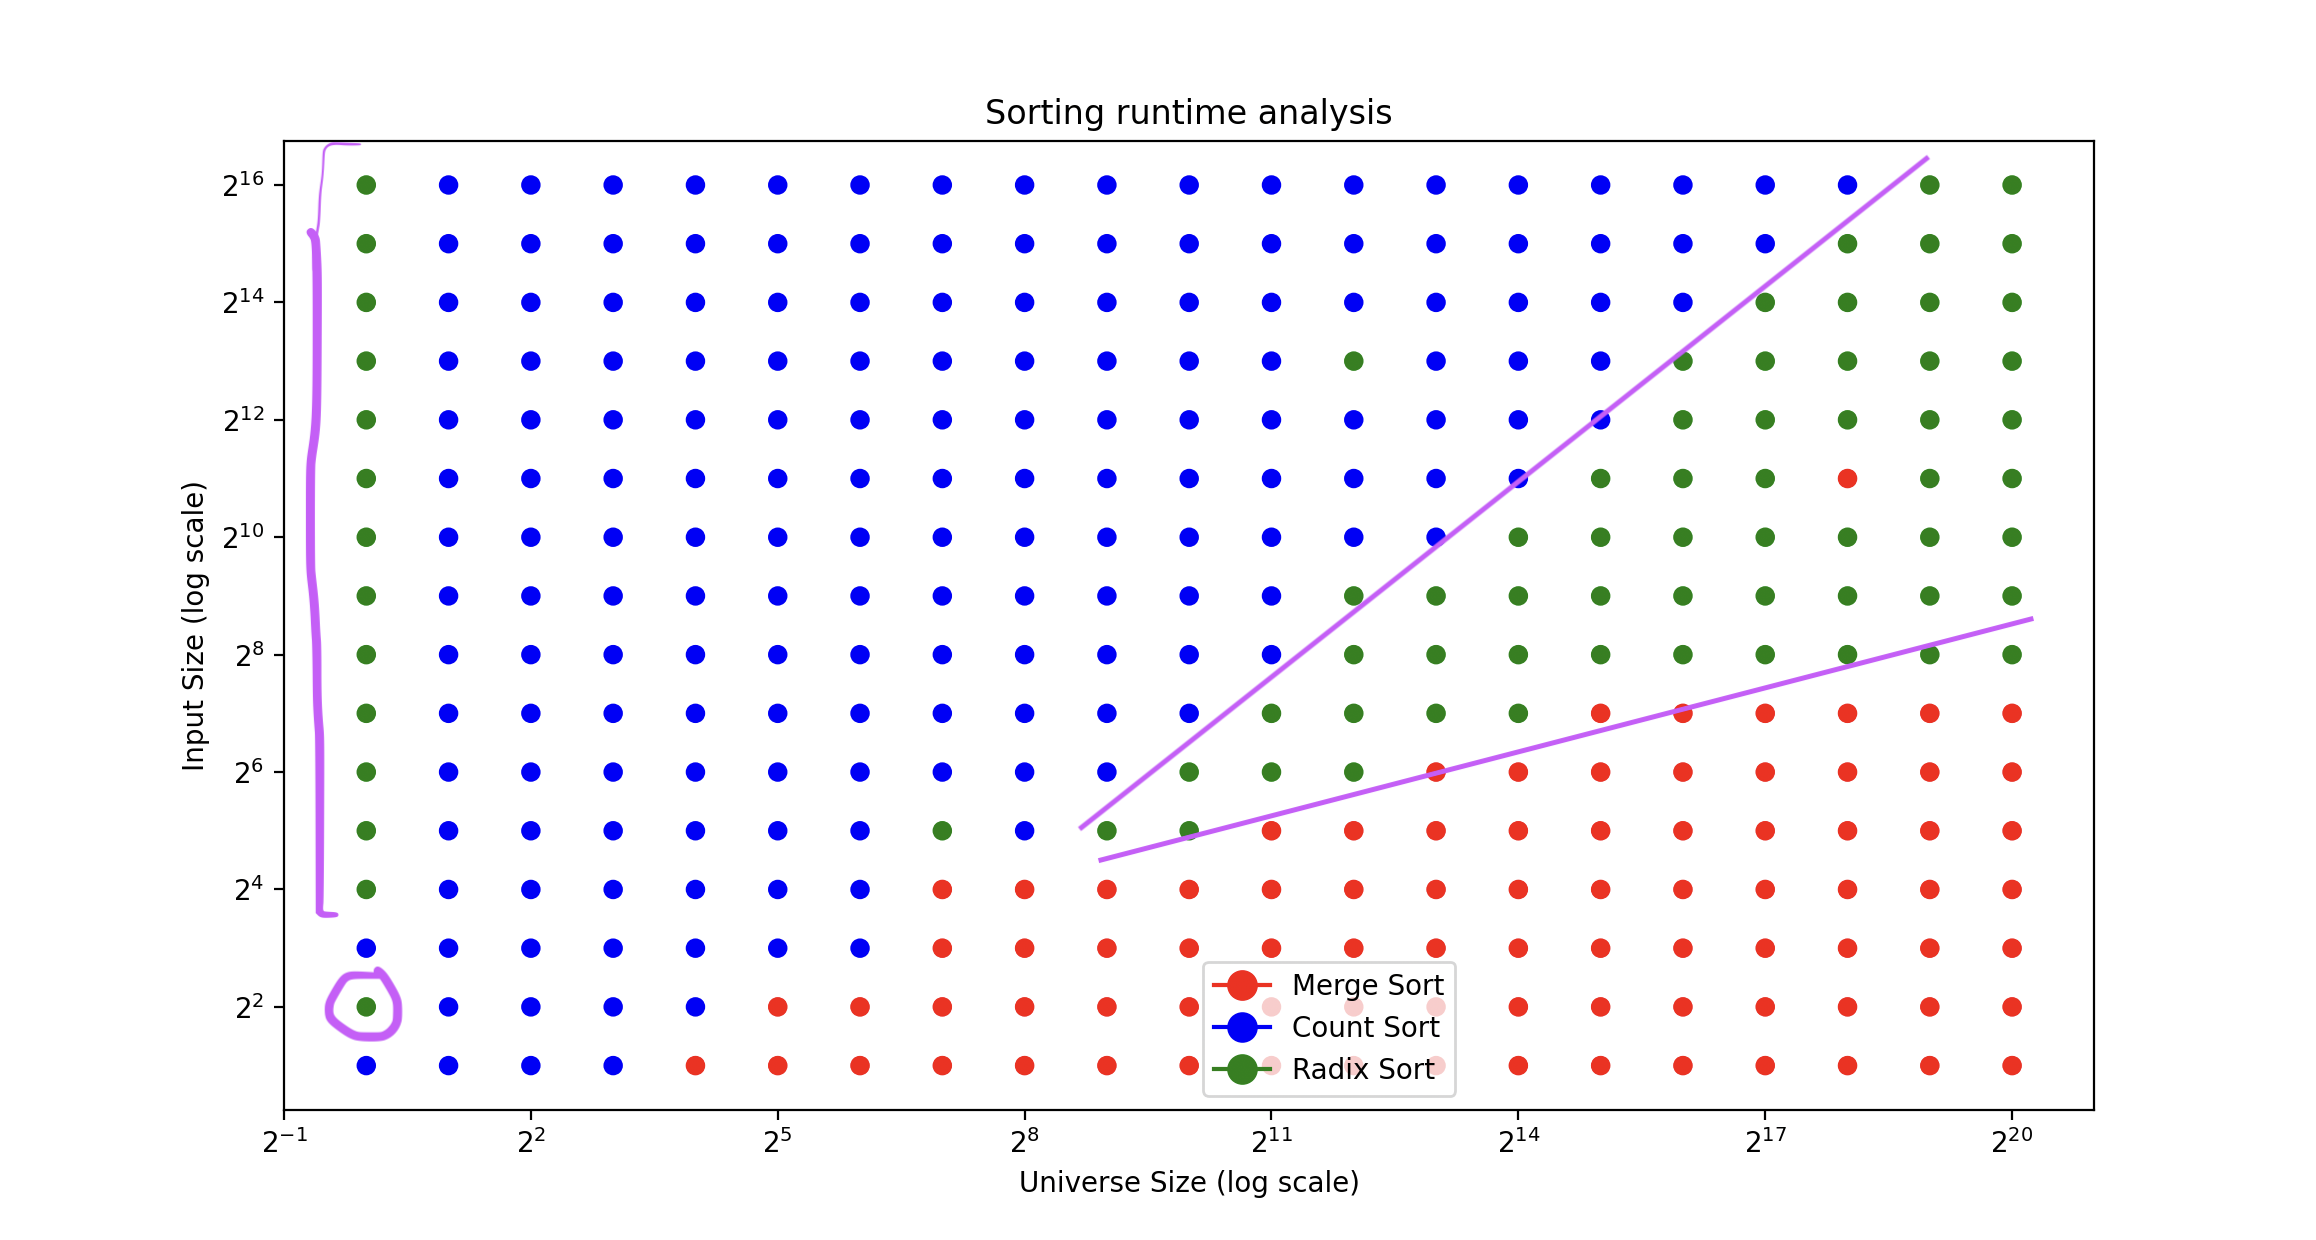
\includegraphics[scale=0.35]{graphs/sort_analysis.png}
        \newline
        Yes, the output graphed above is consistent with what is expected by algorithmic analysis. \CountingSort dominates for high input size, \MergeSort dominates for high universe size, and \RadixSort wins the area in-between the two. Interestingly, \RadixSort seems to also have some outlier cases that encroach on count sort along the input size axis for a very small universe.
    \end{quote}
        \end{enumerate}

\end{enumerate}
\end{document}
